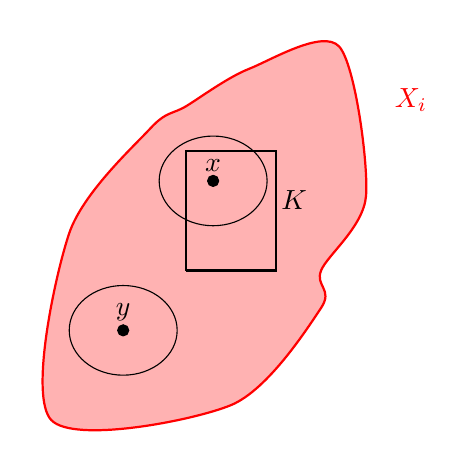
\begin{tikzpicture}
    \begin{axis}[
        axis x line=none,
        axis y line=none,
        %width=9cm,
        %height=4.5cm,
        xmin= 0,     % start the diagram at this x-coordinate
        xmax= 5,     % end   the diagram at this x-coordinate
        ymin= 0,     % start the diagram at this y-coordinate
        ymax= 5,     % end   the diagram at this y-coordinate
        xlabel=$Y$,
        ylabel=$X$,
        ticks=none,
        enlargelimits=true]

        \addplot[mark=none, red, smooth cycle, thick, fill=red!30] coordinates {(0,0) (2,0.2) (3,1.5) (3,2) (3.5,3) (3.2, 5) (2.2, 4.7) (1.5, 4.2) (1.1, 3.9) (0.2, 2.5)};
        \node[red] at (axis cs:4,4) [anchor=south] {$X_i$};

        % Draw solid square
        \addplot[mark=none, thick] coordinates {(1.5,2.0) (2.5,2.0) (2.5,3.6) (1.5,3.6) (1.5,2.0)};
        \node at (axis cs:2.7,3.2) [anchor=90] {$K$};


        % Draw x and annotation
        \node at (axis cs:1.8,3.2) [anchor=-90] {$x$};
        \draw (axis cs:1.8,3.2) circle[radius=0.6];
        \addplot[mark=*] coordinates {(1.8,3.2)};

        \node at (axis cs:0.8,1.2) [anchor=-90] {$y$};
        \draw (axis cs:0.8,1.2) circle[radius=0.6];
        \addplot[mark=*] coordinates {(0.8,1.2)};
    \end{axis} 
\end{tikzpicture}
